\subsection{Calculating the total enhancement}

To get the total enhancement in the square simulated area (see figure~\ref{fig:symmetry}) the $\mathbf{|E|}^4$ approximation in equation \ref{eq:enhancement} was used. The measured enhancement of this area is the mean of the values within the slice.

\begin{figure}[!h]
  \centering
  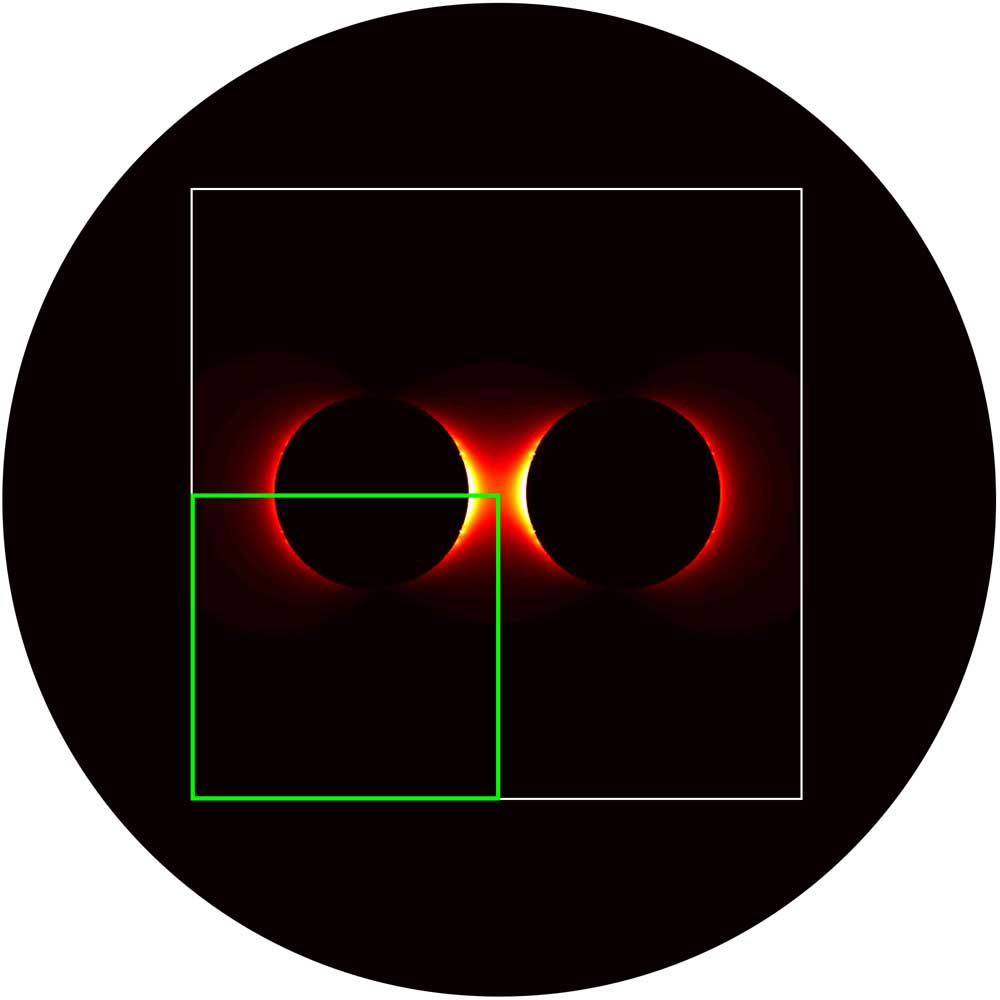
\includegraphics[width=0.5\textwidth]{./images/fwhm-chart.jpg}
  \caption{The simulated square area (green box) compared to the calculated area (white box) compared to the total area measured by the laser (approximated as circle). The laser has a fwhm of \SI{570}{nm} according to \cite{heeg}.}
  \label{fig:symmetry}
\end{figure}

The average value is $60.2$ for the \SI{2}{nm} corner size, $60.2$ for the \SI{5}{nm} corner size (both in the plane of graphene) and $59.2$ for the \SI{5}{nm} corner size for a planar slize at $z=\SI{40}{nm}$. The similarity between these values shows that the estimation of ref.~\cite{heeg} to use the $z=\SI{40}{nm}$ plane is surprisingly accurate.

There is one last factor be taken into account: The used laser spot with a fwhm of \SI{570}{nm} can be estimated by a circle of radius \SI{285}{nm}. The simulated area of \SI{160 000}{nm^2} just accounts for $62.7\%$ of the area of the laser spot. As the Raman signal arises from the area of the entire laser spot, the calculated total enhancement decreases when accounting for this area (see figure~\ref{fig:symmetry}).

The area around the simulated area is approximated as the mean of the outer points of the simulated area.

Taking the laser geometry into account the resulting enhancement values are $38.1$ for the \SI{2}{nm} corner radius, $37.8$ for the \SI{5}{nm} corner radius (both in the plane of graphene) and $37.2$ for the \SI{5}{nm} corner radius for a planar slice at $z=\SI{40}{nm}$. This confirms the exponential enhancement as a function of the calculated near field intensity within the cavity depicted in ref.~\cite{heeg}.

\subsection{Spatial coherence in near-field Raman scattering}

Classical Raman scattering is treated as a spatially incoherent process which means that spatially distinct locations are considered to be uncorrelated and the scattered signal is proportional to the scattering volume. A recent publication suggested that at the nanoscale this assumption does not hold and there is a correlation length of about \SI{30}{nm} for Raman scattering in graphene \cite{coherence}.

To account for this effect the outgoing enhancement has to be adapted. The easiest approximation is to take the mean of a radius of \SI{30}{nm} around each point instead of the point's value directly for the outgoing enhancement, effectively blurring the slice as shown in figure~\ref{fig:coherence}. From the incoming and outgoing enhancement, the total enhancement can be calculated as\cite{maier2007}

\begin{equation}
  Enh_\mathrm{loc}(\mathbf{r},\omega_L)=\frac{\left|\mathbf{E}_\mathrm{loc}(\mathbf{r}, \omega_L)\right|^2}{\left|\mathbf{E}_0\right|^2}\frac{\left|\mathbf{E}_\mathrm{loc}(\mathbf{r}, \omega_L-\omega_\mathrm{ph})\right|^2}{\left|\mathbf{E}_0\right|^2}.
\end{equation}

Taking this approximation into account for the \SI{40}{nm} slice the total enhancement decreases from $37.2$ to $23.0$ which almost matching the measured value of $12.8$ from ref.~\cite{heeg}.

\begin{figure}[!h]
  \centering
  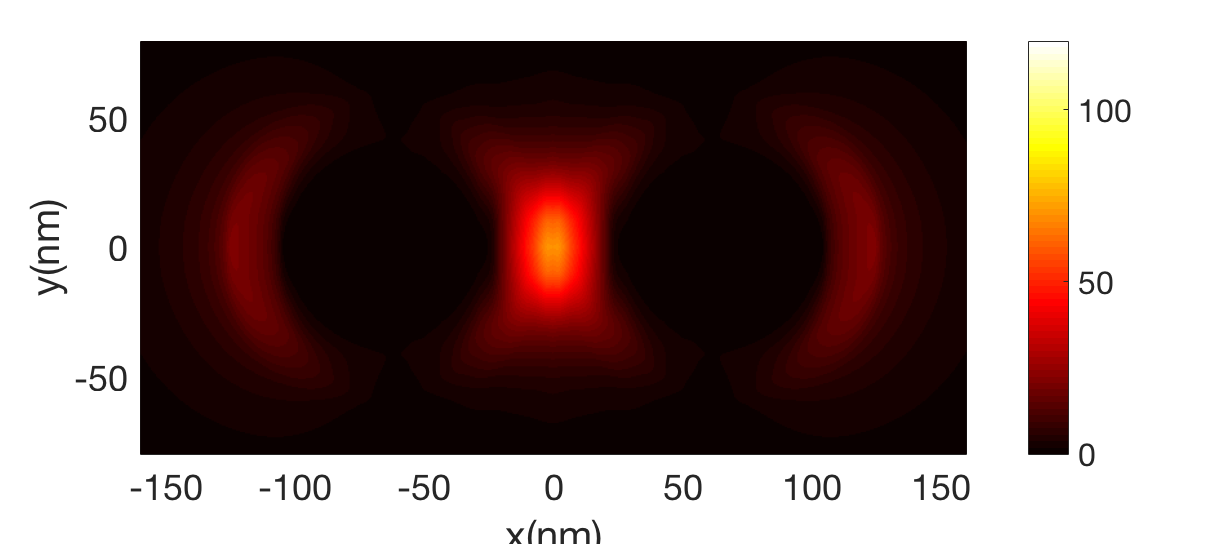
\includegraphics[width=0.8\textwidth]{./images/coherence.png}
  \caption{Outgoing local enhancement for a $z=\SI{40}{nm}$ slice. Due to the spatial coherence effect in near-field Raman scattering the outgoing enhancement is effectivly blurred with a radius of \SI{30}{nm} which decreases the total enhancement.}
  \label{fig:coherence}
\end{figure}
